
\documentclass[12pt]{report}
\usepackage[a4paper]{geometry}
\usepackage[myheadings]{fullpage}
\usepackage{fancyhdr}
\usepackage{lastpage}
\usepackage{graphicx, wrapfig, subcaption, setspace, booktabs}
\usepackage[T1]{fontenc}
\usepackage[font=small, labelfont=bf]{caption}
\usepackage{fourier}
\usepackage[protrusion=true, expansion=true]{microtype}
\usepackage[english]{babel}
\usepackage{sectsty}
\usepackage{url, lipsum}
\usepackage{xcolor}
\usepackage{listings}
\usepackage{spverbatim}
\usepackage{hyperref}


\renewcommand{\thesection}{\arabic{section}}
\setcounter{section}{0} %numeracija sekcija

\graphicspath{ {./images/} }
\setlength\parindent{0pt} %nemoj uvuci paragraph
\newcommand{\code}[1]{\texttt{#1}} % code u tekstu

%color
\definecolor{my_green}{rgb}{0.027, 0.663, 0.545}
\newcommand{\mygreen}[1]{{\color{my_green}#1}}
\definecolor{my_red}{rgb}{0.843, 0.000, 0.384}
\newcommand{\myred}[1]{{\color{my_red}#1}}


%---- CODE LISTING
\definecolor{codecomment}{rgb}{0.561, 0.561, 0.561}
\definecolor{codegray}{rgb}{0.5,0.5,0.5}
\definecolor{codepurple}{rgb}{0.58,0,0.82}
\definecolor{pozadina}{rgb}{0.925, 0.925, 0.925,}


\lstdefinestyle{mystyle}{
    backgroundcolor=\color{pozadina},   
    commentstyle=\color{codecomment},
    keywordstyle=\color{magenta},
    numberstyle=\tiny\color{codegray},
    stringstyle=\color{codepurple},
	basicstyle=\ttfamily\footnotesize,
    breakatwhitespace=false,         
    breaklines=true,                 
    captionpos=b,                    
    keepspaces=true,                 
    numbers=left,                    
    numbersep=3pt,                  
    showspaces=false,                
    showstringspaces=false,
    showtabs=false,                  
    tabsize=2
}
\lstset{style=mystyle}
%--------



\begin{document}

\newcommand{\HRule}[1]{\rule{\linewidth}{#1}}
\onehalfspacing


%-------------------------------------------------------------------------------
% HEADER & FOOTER
%-------------------------------------------------------------------------------
\pagestyle{fancy}
\fancyhf{}
\setlength\headheight{15pt}
\fancyhead[L]{CANAL PLUS}


%-------------------------------------------------------------------------------
% FIRST PAGE
%-------------------------------------------------------------------------------
\title{ \normalsize \textsc{CANAL PLUS}
\\ [1.0cm]
\HRule{0.5pt} \\
\LARGE \textbf{\uppercase{DOCKER LOCAL REGISTRY}}
\HRule{2pt} \\ [0.5cm]
\normalsize  \vspace*{5\baselineskip}

\includegraphics[scale=0.8]{logo_rtrk.png}
}



\author{Miroslav Blazic}
\date{\today\\
	\fbox {Version: v1.0}
}

\maketitle



%-------------------------------------------------------------------------------
% TABLE OF CONTENT
%-------------------------------------------------------------------------------
\newpage
\tableofcontents
\newpage




\section*{ABSTRACT}
Pisi ponekad dva tri reda.
\newpage


\section{INTRODUCION}

\begin{center}
	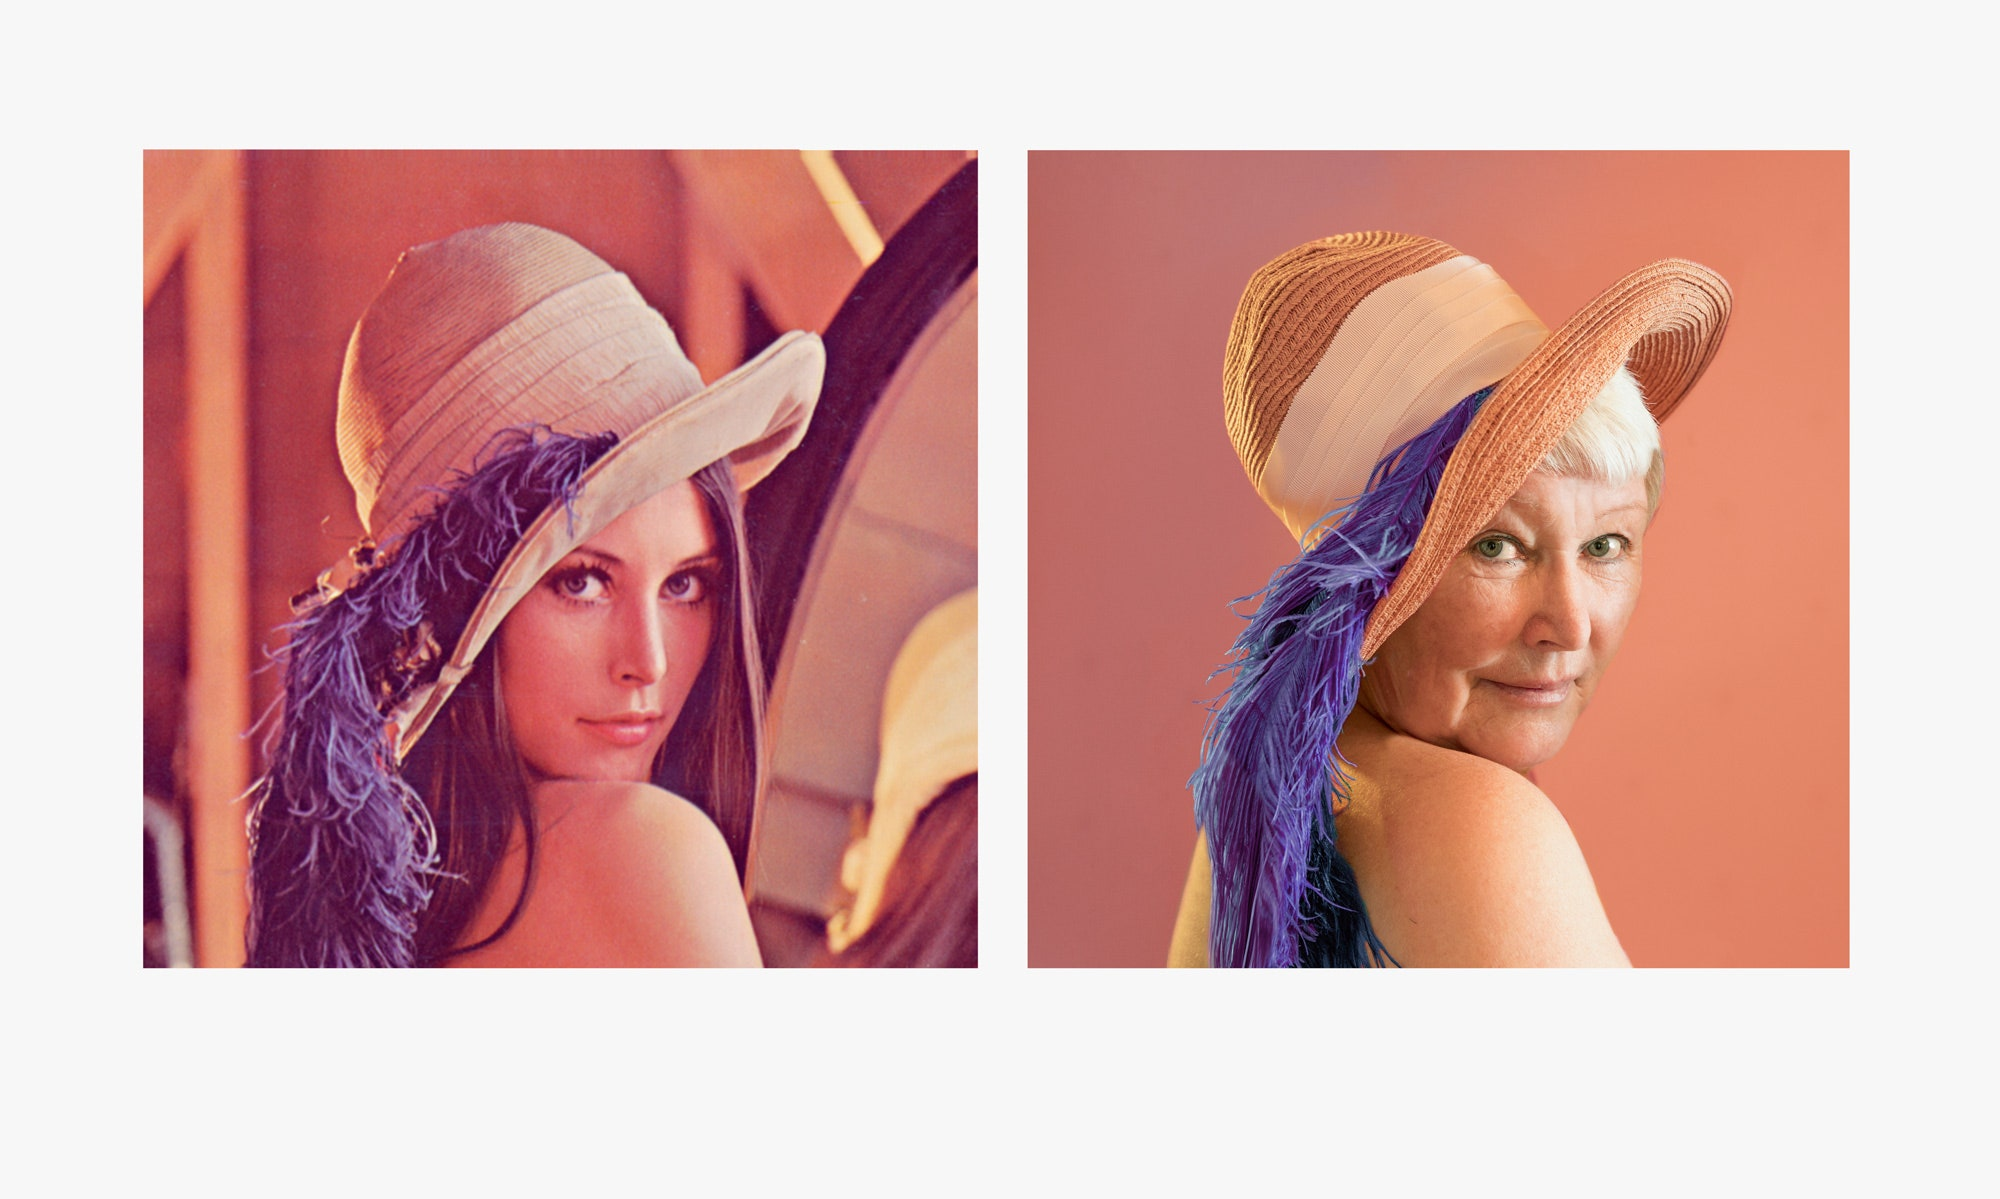
\includegraphics[scale=0.25]{introduction1.png}
\end{center}



Pisi ponekad dva tri reda.
\newline
Pisi ponekad dva tri reda.
\newline


\mygreen{Recenicu pocinjemo sa zelenom bojom} a zavrsavamo sa default.
\myred{Crvena boja} default.



\section{NASLOV}
Pisi ponekad dva tri reda.

Linkuj nesto:
%\url{https://www.google.com/.

\subsection{PODNASLOV}
Pisi ponekad dva tri reda.
\newline
DONJA{\_}CRTA
\newline
Tekstualni kod \code{probaj ovako}
\begin{lstlisting}[language=C, caption= Opis liste.]
	Pisi ponekad dva tri koda.
	Pisi ponekad dva tri koda.
	Pisi ponekad dva tri koda.
\end{lstlisting}





\end{document}